\section{Results}

\subsection{The preregistered FINAL-5J execution completed without operational failure}

The final run completed all \FinalEmbeddings{} embeddings and \FinalEvaluations{} channel evaluations (\FinalTasks{} planned tasks) under the frozen \code{FINAL-5J-v1} contract. The main matrix contained 50 pairs and seven methods; the two incremental sweeps used the preregistered 10-pair subset. The final dispatcher reported \code{run\_complete\_local} with \FinalWorkers{} workers. Analysis was built without an incomplete-run override and contained all \FinalEvaluations{} raw rows, zero missing rows, zero invalid rows, and \code{partial\_analysis=false}. Pair-level uncertainty used \FinalBootstrap{} bootstrap repetitions and aggregated repeated attack seeds within pair, method, and condition before inferential comparison.

These completion checks are important because the protocol distinguishes an operational failure from a scientifically valid failure to recover a payload. The former would indicate an execution or environment problem; the latter is an observed outcome of the frozen method under the frozen input and channel contract. No operational failures occurred in the final run.

\subsection{Complete recovery was confined to the clean condition}

The clean condition exposed method-dependent end-to-end validity that was hidden by the earlier pilot experiment. C0, C1, C2, C3\_NP, and C3 each completed \InternalCleanComplete{} clean pairs. The same preregistered pair, \code{coco-000000479126-000000199771}, reached the typed S4 header-failure state for all five internal methods. B1 completed \BOneCleanComplete{} clean pairs. B2 completed \BTwoCleanComplete{} clean pairs; the remaining pairs were retained as S5 extraction/transform scientific failures under the frozen clean-valid candidate contract. Thus the clean outcomes were scientifically heterogeneous even though the execution itself was operationally complete.

None of the attacked conditions produced complete end-to-end recovery for the internal C-family. Across JPEG qualities 90, 70, and 50, Gaussian variances 5, 10, and 15, and salt-and-pepper densities 0.01, 0.03, and 0.05, these methods terminated at S4. B1 behaved differently: all attacked evaluations retained a valid header and partial payload (S2), rather than complete recovery. B2 split consistently between S2 partial recovery and S5 extraction/transform failure, reflecting the same 32/18 pair partition observed in the clean condition. Figure~\ref{fig:5j-failure-stages} summarizes these typed failure modes.

\begin{figure}[t]
\centering
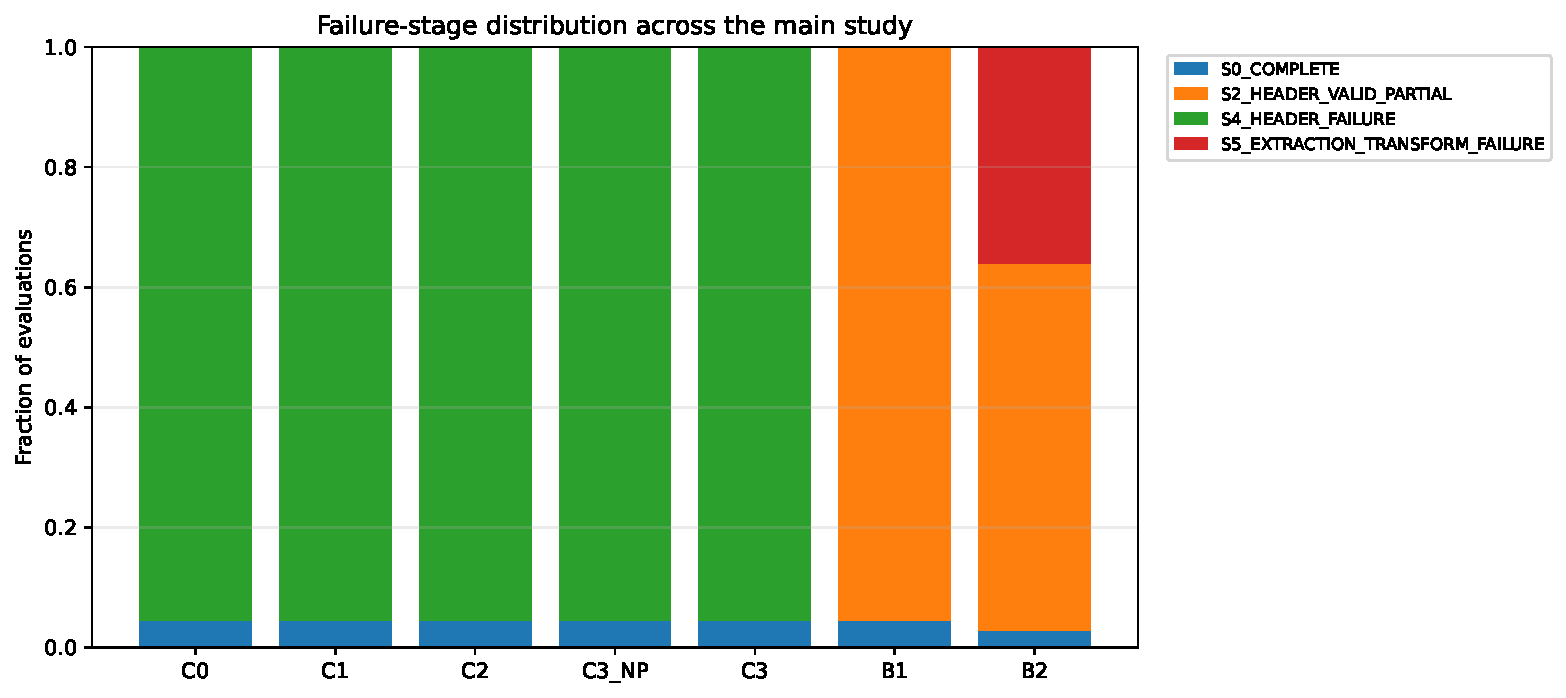
\includegraphics[width=\linewidth]{docs/5j/final-run-20260812/figures/figure_failure_stages.pdf}
\caption{Failure-stage composition in the completed FINAL-5J run. Scientific recovery failures are retained as typed outcomes and are distinct from operational failures, which were zero.}
\label{fig:5j-failure-stages}
\end{figure}

\subsection{The seven-method comparison revealed a robustness--fidelity trade-off}

\begin{table*}[t]
\centering
\caption{Selected pair-level FINAL-5J method summaries generated from the frozen analysis artifact.}
\label{tab:5j-main-summary}
\begin{tabular}{lrrrrrr}
\toprule
Method & Complete recovery & Payload correct & Raw BER & Cover PSNR (dB) & Runtime (s) & Operational failures \\
\midrule
C0 & 0.0980 & 0.1000 & 0.3086 & 45.0000 & 2.3202 & 0 \\
C1 & 0.0980 & 0.1000 & 0.3074 & 45.0000 & 2.3013 & 0 \\
C2 & 0.0980 & 0.1000 & 0.3085 & 45.0000 & 2.3925 & 0 \\
C3\_NP & 0.0980 & 0.1000 & 0.3075 & 45.0000 & 2.2388 & 0 \\
C3 & 0.0980 & 0.1000 & 0.3074 & 45.0000 & 2.2313 & 0 \\
B1 & 0.1000 & 0.7060 & 0.2940 & 45.7188 & 0.0104 & 0 \\
B2 & 0.0640 & 0.6102 & 0.3898 & 44.8942 & 0.0150 & 0 \\
\bottomrule
\end{tabular}
\end{table*}


Table~\ref{tab:5j-main-summary} shows that complete recovery and partial recoverability did not rank the methods in the same way. C3 had a pair-level complete-recovery mean of \CThreeCompleteMean{} and payload-correct mean of \CThreePayloadMean{}. B1 had a similar complete-recovery mean (\BOneCompleteMean{}) but a substantially larger payload-correct mean (\BOnePayloadMean{}) and lower raw BER (\BOneBERMean{}). B2 had lower complete recovery (\BTwoCompleteMean{}) while still retaining a larger partial payload fraction (\BTwoPayloadMean{}) on its defined evaluations.

The blind baselines also yielded directly defined secret-reconstruction quality. B1 produced mean reconstruction PSNR \BOneSecretPSNR{}~dB and SSIM \BOneSecretSSIM{}, whereas B2 produced \BTwoSecretPSNR{}~dB and \BTwoSecretSSIM{}. Reconstruction PSNR is not defined on the same basis for failed internal rows and is therefore not used as a cross-family superiority endpoint.

\subsection{C3 did not improve complete recovery over C0, but reduced raw BER}

The preregistered paired comparison between C3 and C0 found no difference in complete-recovery rate: the mean paired difference was 0.0000, all 50 pairs were ties, and the Holm-adjusted Wilcoxon value was 1.0. Payload-correct fraction was likewise unchanged on the 49 pairs with defined paired values. Raw BER, however, was lower for C3 on every one of those 49 pairs. The mean paired difference (C3 minus C0) was $-0.0012$ with a 95\% bootstrap interval of $[-0.0013,-0.0011]$; the adjusted significance value rounded below $10^{-6}$ in the archived table. Runtime did not differ detectably after multiplicity correction (mean difference $-0.0889$~s; Holm-adjusted $p=1.0$).

Removing the C3 placement component (C3\_NP) also did not change complete recovery. The C3--C3\_NP raw-BER difference was only $-0.0001$ (95\% interval $[-0.0002,-0.0000]$), with Holm-adjusted $p=0.610659$. In this frozen operating regime, the measured end-to-end benefit of the full C3 design is therefore a small BER reduction relative to C0, not an increase in complete-payload recovery.

\begin{figure}[t]
\centering
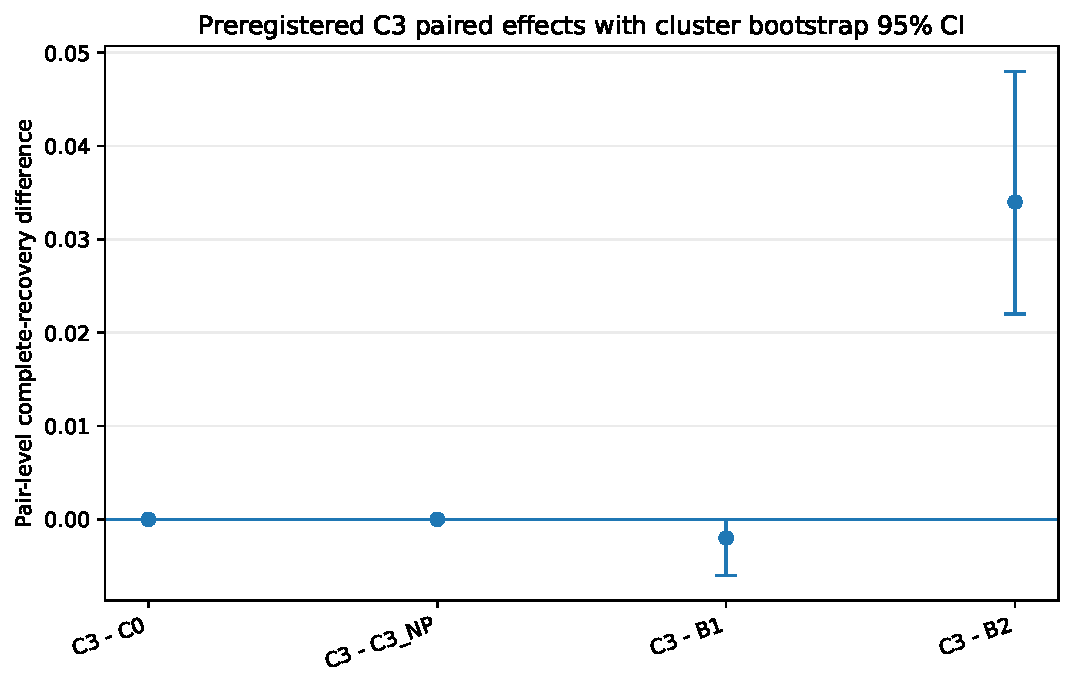
\includegraphics[width=\linewidth]{docs/5j/final-run-20260812/figures/figure_primary_complete_recovery_effects.pdf}
\caption{Preregistered paired effects for complete recovery. C3 ties C0 and C3\_NP on this endpoint, differs little from B1, and exceeds B2 because B2 fails clean extraction on 18 of the 50 pairs.}
\label{fig:5j-primary-complete}
\end{figure}

\subsection{Comparisons with B1 and B2 separate complete validity from partial recoverability}

Against B1, C3 showed essentially the same complete-recovery endpoint (mean difference $-0.0020$; 49 ties and one pair favouring B1; Holm-adjusted $p=1.0$), but substantially less partial payload recovery: the mean payload-correct difference was $-0.6055$ on 49 defined pairs. C3 also had a raw-BER mean 0.0129 higher than B1 on those pairs. B1 was much faster computationally (mean 0.0104~s versus 2.2313~s for C3), although the methods implement different transport structures and this runtime difference should not be interpreted independently of functionality.

Against B2, C3 had a higher complete-recovery mean by 0.0340. Seventeen pairs favoured C3 and 33 tied, yielding Holm-adjusted $p=0.000411$. On the 32 pairs for which both methods had defined payload/BER comparisons, C3 recovered a smaller payload fraction (mean difference $-0.5102$) but had lower raw BER (mean difference $-0.0822$). These apparently opposing directions are not contradictory: complete validity, partial payload fraction, and raw BER describe different aspects of transport behaviour and must be reported together.

Figure~\ref{fig:5j-complete-recovery} and the archived payload-recovery figure provide the corresponding method-level view. The complete numerical tables, pair-level rows, raw 8,420-row evaluation table, and analysis checksums are versioned with the result snapshot used for this manuscript.

\begin{figure}[t]
\centering
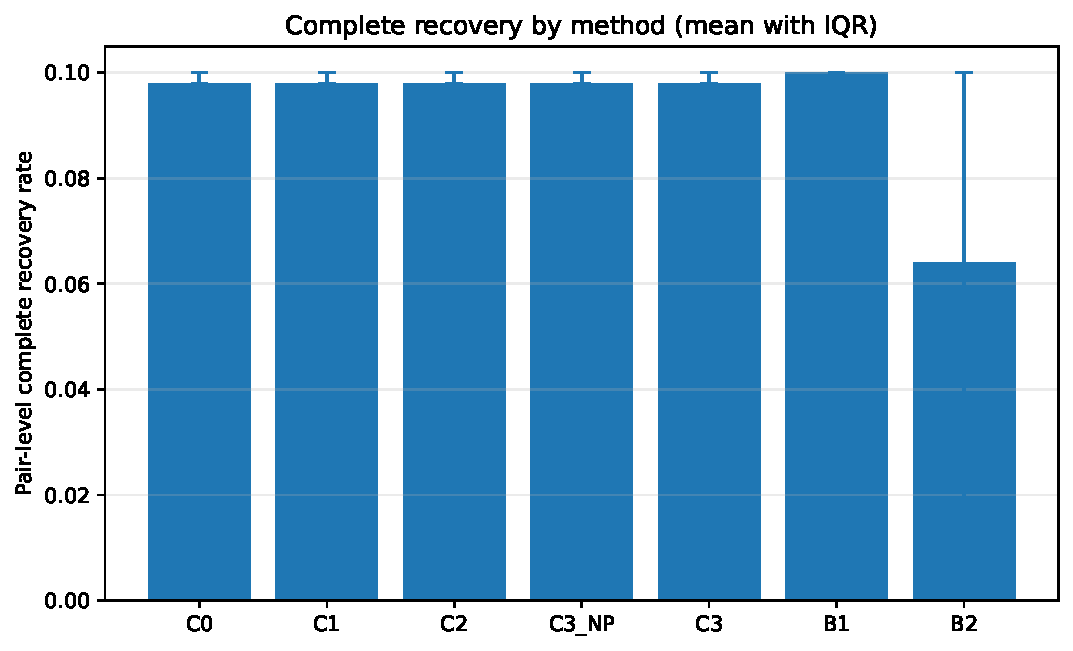
\includegraphics[width=\linewidth]{docs/5j/final-run-20260812/figures/figure_complete_recovery.pdf}
\caption{Pair-level complete-recovery summary for the seven FINAL-5J methods. Complete recovery is concentrated in the clean condition; attacked outcomes are represented separately through typed failure stages and partial-payload metrics.}
\label{fig:5j-complete-recovery}
\end{figure}
